\documentclass{article}

\usepackage[english]{babel}

% Set page size and margins
% Replace `letterpaper' with `a4paper' for UK/EU standard size
\usepackage[letterpaper,top=2cm,bottom=2cm,left=3cm,right=3cm,marginparwidth=1.75cm]{geometry}

\usepackage{amsmath}
\usepackage{graphicx}
\usepackage[colorlinks=true, allcolors=blue]{hyperref}

\title{Bézier Curves and Computational Approaches}
\author{Jacob LeBlanc}

\begin{document}
\begin{titlepage}
\maketitle
\begin{center}
    \Large
    \textbf{Abstract}
\end{center}
\large
This paper seeks to outline the basics of Bézier curves. It begins by introducing Bézier curves and describing some of the features which make them useful. Then, it touches on the author's relevant personal experience which contributes to their interest and understanding of this topic. It will then discuss the mathematical history which led to the development of Bézier curves. Then, key properties and definitions of the Bézier curve will be discussed. The following section will describe some useful algorithms used for defining and modifying Bézier curves. This paper will then explore the computational methods used to create and modify Bézier curves, with examples of potential implementations of these algorithms and their time complexity. Finally, it concludes with a look at real world use cases for Bézier curves.
\end{titlepage}


\section{Introduction}
Bézier curves are parametric equations defined by a set of control points, which exercise "pull" over the shape of the curve without necessarily falling on the curve. Bézier curves are the foundation of vector graphics and hold special relevance to computer graphics. Being defined by an algorithm and a small set of control points gives this approach rather than a grid of pixels, as in rasterized graphics, creates perfect curves on any size screen and any resolution. Some prominent use cases for Bézier curves are graphic design and font definitions. These curves are also useful for other applications which require an analog of exactly defined movement over irregular curves, for example: physics simulations and trajectories for the movement of robotics.

\begin{figure}[h]
    \centering
    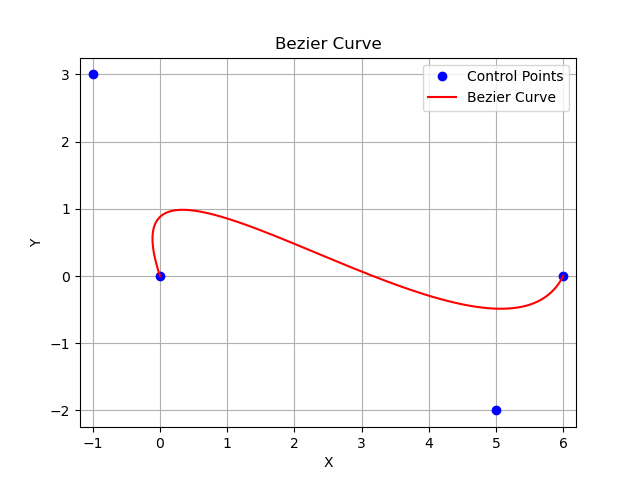
\includegraphics[width=0.5\linewidth]{Ex-Curve.png}
    \caption{An example Bézier curve with 4 control points}
    \label{fig:enter-label}
\end{figure}

\section{Relevant Courses}
This section gives a general idea of the author's background knowledge, and the ways it informed the choice of topic and approach towards it.

\subsection{Computer Science Background}
As a computer science and math double major, I have extensive experience with programming, algorithms, and computational problem solving. It is hard to list a single course as exactly relevant to this work, but Computer Science 1 and 2 (CS-1440 and CS-2440 respectively) are the most pertinent level of understanding necessary to replicate this paper. My experience with a CS-1440 equivalent introduced me to basic programming, control structures, and the Python programming language, which I make use of in this paper.

\subsection{Computational Mathematics}
MAT-2310, or computational mathematics, was relevant to this analysis as it allowed me a greater understanding of efficient and error-reducing approaches towards computationally solving mathematical problems. This course also gave me an opportunity to further dive into Python and familiarize myself with the packages relevant for mathematical applications.

\subsection{Numerical Methods}
MAT-4310, or numerical methods, allowed me to gain additional insight into the application of computation towards mathematics. This course emphasized analysis of error, computational complexity, and numerical stability. My experience in this course afforded me a greater depth of understanding in the topics touched on in MAT-2310, creating the foundation needed for the work inherent to this paper.

\pagebreak

\section{Historical Background}
\subsection{Bernstein Polynomials}
The foundations of Bézier curves lay in Bernstein polynomials. In 1912, Sergei Natanovich Bernstein introduced a technique of approximating curves by using a linear combination of basis polynomials in the form:$$B(x)=\sum_{i=0}^nf(\frac{i}{n})\beta_{n,i}(x)$$ where the left hand side is called the Bernstein polynomial of degree $n$ \cite{bernstein-polynomials}. The right hand side of the equation consists of the sum of the basis polynomials, which themselves are composed of a Bernstein coefficient ($f(\frac{i}{n})$) and a basis polynomial ($\beta_{n,i}(x)=\binom{n}{i}x^i(1-x)^{n-i}$). This sequence converges uniformly to a function $f$ on the interval $x\in[0,1]$ so long as f is continuous on this interval \cite{bernstein-polynomials}. Thus, the Bernstein polynomial approximates $f$. A special case of this approach, where the coefficient is instead defined by a set of control points and B is a parametric function, will form the analytical basis of Bézier curves.

\subsection{de Casteljau's Innovation}
 However, while these approximations were useful to Bernstein in creating a constructive proof to the Weierstrass approximation theorem, they did not see much other use until 1959. That is when Paul de Casteljau, a French mathematician working at car manufacturer Citroen, created a recursive method of evaluating parametric polynomials in Bernstein form. His algorithm takes an $n$ degree Bézier curve in standard Bernstein form, and evaluates it at point $t$. This approach allowed de Casteljau to evaluate a curve in a more practical manner, as it could reduce the degree of terms being calculated when compared to evaluating the full sum of a Bernstein polynomial. It also came with the benefit of allowing a curve to be split into two curves at an arbitrary point. His algorithm additionally improved numerical stability by reducing the amount of arithmetic required per iteration as compared to direct Bernstein evaluation.\cite{shene11} This paper will discuss the actual algorithm in section 5.

\subsection{Bézier's role}
de Casteljau's algorithm would be put to use in the 1960s by Pierre Bézier, an engineer at rival car company Renault, who utilized the algorithm to create smooth curves for computer graphics and car design. Utilizing this algorithm made calculations of Bernstein approximations practical for the computer hardware of the day, as precision could be sacrificed to reduce the number of computations in the approximation. Bézier's unique approach was in utilizing Bernstein polynomials to define parametric equations, and in doing so pioneering the use of "control points" (sometimes called "Bézier points") for defining deformations of a parametric curve. His perspective was that maintaining precision through the process of industrial design required a simpler approach than explicit curve definitions which left room for error during modification; for this reason, Bézier chose to instead "[inscribe] a so-called ‘basic’ curve, with the appropriate shape, in a cube," where the cube, acting as a reference frame, would undergo linear transformations in order to modify the basic curve inscribed within \cite{rabut02}. In this paper, the curves analyzed lay on a plane for simplicity's sake, rather than within a cube.

\pagebreak

\section{Properties of Bézier Curves}
Given a set of control points $P_0, P_1, \dots, P_n$, the Bézier curve is defined as a Bernstein polynomial: $$B(t)=\sum_{i=0}^n\beta_{n,i}(t)P_i$$ where the basis polynomials are defined as: $$\beta_{n,i}(t)=\frac{n!}{i!(n-i)!}t^i(1-t)^{n-i}$$ \cite{shene11}


\subsection{Degree of the Curve}
Note that in the above definition of the basis polynomial, given $n+1$ polynomials, the degree of the parameter $t$ is $i + (n-i) = n$. Thus, given $n+1$ control points, the Bézier curve will be of degree $n$ \cite{shene11}.

\subsection{Starting and Ending Control Points}
Any given Bézier curve must pass through the control points $P_0$ and $P_n$, and indeed begins and ends at those points. 

Note that for $i=0$, the basis function $\beta_{n,i}(t)=\frac{n!}{n!}t^0(1-t)^n=(1-t)^n$. Given this, one can see that at $t=0$ and $i=0$, $$\beta_{n,i}(0)*P_0 = 1*P_0 = P_0$$
Additionally note that for $i=n$, the basis function $\beta_{n,i}(t)=\frac{n!}{n!}t^n(1-t)^0=t^n$. Given this, notice that for $t=1$ and $i=n$, $$\beta_{n,i}(1)*P_n=1*P_n=P_n$$
Therefore, any given Bézier curve $B(t)$ must start by passing through $P_0$ and end by passing through $P_n$

\subsection{Domain of the Parameter}
Note that the parameter $t$ has the domain restriction $t\in[0,1]$, where $t=0$ corresponds to $P_0$ and $t=1$ to $P_n$. If the domain is given as some other values, perhaps $t\in[a,b]$, then a change of variables is required, using the formula $\hat{t}=\frac{t-a}{b-a}$ and substituting $\hat{t}$ for $t$ in each basis function \cite{shene11}.

\subsection{Partition of Unity}
Note that since $t\in[0,1]$, and $0 \leq i \leq n$, then any given basis function is greater than $0$. Also, by the binomial theorem, one can say that $$\sum_{i=0}^n\beta_{n,i}(t)=\binom{n}{i}t^i(1-t)^{n-1}=(t+(1-t))^n=1$$ \cite{wyss-gallifent21}
Given these two points of information, one must conclude that any given basis function, $\beta_{n,i}(t)\in[0,1]$ is true. Because all of these functions are in the range $[0,1]$, and sum to $1$, they represent a way of partitioning $1$ into $n+1$ intervals. Therefore, the basis functions can be treated as weights in a weighted average of the control points\cite{shene11}. As Dr. C-K Shene of MTU puts it: "we could say "to compute [$B(t)$], one takes the weight [$\beta_{n,i}(t)$] for control point [$P_i$] and sum them together."

\subsection{Convex Hull}
The Bézier curve given by $n+1$ control points must lay entirely within the convex hull of those control points.\cite{shene11}\cite{wyss-gallifent21} The convex hull of the control points is the "smallest convex set that contains all [the control points].\cite{shene11} This property is useful as it defines definite, computable bounds for whatever curve is being generated. \cite{shene11}

\subsection{Linear Transformations and Invariance}
One of the primary goals Bézier had in defining these curves was to reduce error during modification of curves. This property is fulfilled, as any linear transformation $T$ applied to the final curve $B(t)$ is equivalent to applying $T$ to the control points $P_i$ and then constructing the curve. This is because $B(t)$ is constructed via a linear combination of the control points and $T$ is also linear.\cite{wyss-gallifent21} Additionally, any affine or geometric transformations follow this same principle, and can be achieved by transforming the control points rather than the curve.\cite{shene11} This reduces computational complexity and opportunity for error.

\pagebreak

\section{Relevant Algorithms}
Aside from direct Bernstein evaluation, there are several algorithms which are useful for constructing, manipulating, and modifying Bézier curves. The following are some of the most pertinent for general use.

\subsection{de Casteljau's Algorithm}
The most useful and famous algorithm for Bézier curves is de Casteljau's. It presents a geometric method of evaluating Bernstein polynomials with "excellent numerical stability"\cite{hanik-yazdani-tycoqicz24}, and it allows one to evaluate a Bézier curve at a point. This algorithm can be expressed as such:
Given control points $P_0, P_1, \dots, P_n$, the value of the corresponding Bézier curve $B(t)$ at $t\in[0,1]$ can be found using the following rules. $$B_i^0 := P_i$$$$B_i^r := (1-t)B_i^{r-1}(t)+tB_{i+1}^{r-1}(t)$$
Where:
$$r=1,\dots,n$$ $$i=0,\dots,n-r$$
\cite{hanik-yazdani-tycoqicz24}
In other words, one starts with a set of $n+1$ control points. Then, one divides the line segment drawn directly between two of these points with a ratio of $t$ on one side and $1-t$ on the other.\cite{shene11} Continue to perform this operation on all of the control points. This results in a new set of $n$ points. Perform this operation again with these new points as the input, and repeat again with the resulting set of points until only a single point is returned. This final point is the value of $B(t)$ for whatever value of $t$ was given. Find below an illustration of this recursive process courtesy of Dr. C-K Shene:

\begin{figure}[h]
    \centering
    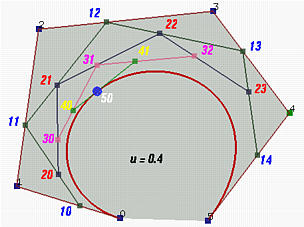
\includegraphics[width=0.5\textwidth]{de-casteljau.jpg}
    \caption{A visual example of de Casteljau's algorithm locating a point along a Bézier curve}
    \label{fig2:de-casteljau}
\end{figure}

Another useful application of de Casteljau's algorithm is splitting a Bézier curve into several Bézier curves at a given parameter $t$. If the original curve was of degree $n$, the resulting curves will also both be of degree $n$. This application can be achieved by performing the full calculation of a point using the algorithm, and then finding the points $B_0^0, B_1^1, B_2^2, \dots, B_n^n$ which act as the left curve's control points. Then, find the points $B_n^n, B_n^{n-1}, B_n^{n-2}, \dots, B_n^0$\cite{pat-mae-cho09}, which act as the right curve's control points.\cite{shene11} Thus, the curve has been split and can now be manipulated in new ways. This approach can also "[compute] the intersection of two Bézier curves," and "[render] Bézier curves
".\cite{shene11}

\subsection{Degree Elevation Algorithm}
It can sometimes be useful to add additional control points to a Bézier curve without modifying the existing shape. This can be advantageous as it allows for finer control over the curve when modifying it later on. To modify a Bézier curve $B(t)$ from $n$ degree to $n+1$, we generate $n+2$ new control points using the following formula: $$P_i^{n+1} = \frac{i}{n+1}P_{i-1}^n+(1-\frac{i}{n+1})P_i^n$$ Where: $$i=0,\dots,n+1$$
\cite{pat-mae-cho09}

More generally, an $n$ degree Bézier curve may be elevated to $n+r$ degree via the formula:
$$P_i^{n+r}=\sum_{j=max(0,i-r)}^{min(n,i)}\frac{\binom{n}{j}\binom{r}{i-j}}{\binom{n+r}{i}}P_j^n$$ Where: $$i=0,1,\dots,n+r$$
\cite{pat-mae-cho09}

\pagebreak

\section{Algorithm Implementations and Analysis}
Below is an implementation in Python of Bézier Curves via direct Bernstein polynomial evaluation. It also includes code to view the plot, and an example using a cubic Bézier curve.
\begin{verbatim}

    import numpy as np
    import matplotlib.pyplot as plt
    from scipy.special import comb

    def Bézier_curve(control_points, num_points):
        n = len(control_points) - 1
        t = np.linspace(0, 1, num_points)
        curve = np.zeros((num_points, 2))

        for i in range(num_points):
            x_coord = 0
            y_coord = 0
            for k in range(n + 1):
                x_coord += comb(n, k) * (1 - t[i])**(n - k) * t[i]**k * control_points[k][0]
                y_coord += comb(n, k) * (1 - t[i])**(n - k) * t[i]**k * control_points[k][1]
            curve[i] = [x_coord, y_coord]
    
        return curve

    def plot_Bézier_curve(control_points, curve_points):
        plt.plot(control_points[:,0], control_points[:,1], 'bo-', label='Control Points',
                 linestyle='None')
        plt.plot(curve_points[:,0], curve_points[:,1], 'r-', label='Bézier Curve')
        plt.title('Bézier Curve')
        plt.xlabel('X')
        plt.ylabel('Y')
        plt.legend()
        plt.grid(True)
        plt.axis('equal')
        plt.show()

    # Example control points
    control_points = np.array([[0, 0], [1, 3], [2, -3], [6,4]])

    # Generate Bézier curve
    curve_points = Bézier_curve(control_points, 100)

    # Plot Bézier curve
    plot_Bézier_curve(control_points, curve_points)

\end{verbatim}

This is the plot output by the above:
\begin{figure}[h]
    \centering
    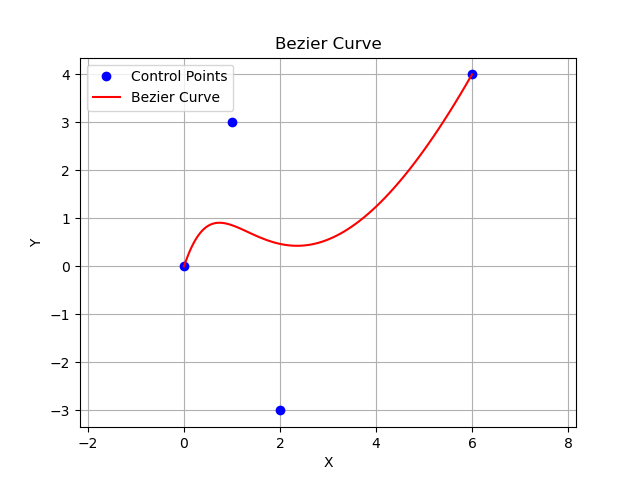
\includegraphics[width=0.5\textwidth]{Cubic-Bern-Bez.png}
    \caption{A cubic Bézier curve via Bernstein Polynomials}
    \label{fig1:cubic-bez}
\end{figure}

This approach is highly functional, but it is not universally applicable. While efficient, executing in roughly linear time when scaling up control points or accuracy, it requires the evaluation of the full sum of basis polynomials. Thus this more efficient algorithm may end up taking more time than creating a curve via de Casteljau's with fewer points but still reasonable accuracy. It also requires evaluation of $n$ degree exponents, which may be difficult on certain CPU architectures. 

Find below an example implementation of de Casteljau's algorithm for evaluating a single point on a Bézier curve:
\begin{verbatim}
    def de_casteljau(control_points, t):
    n = len(control_points) - 1
    points = [point[:] for point in control_points]  # Copy of control points
    for r in range(1, n + 1):
        for i in range(n - r + 1):
            points[i] = [(1 - t) * points[i][0] + t * points[i + 1][0],
                         (1 - t) * points[i][1] + t * points[i + 1][1]]
    return points[0]

    # Usage example
    control_points = np.array([[0, 0], [1, 3], [2, -3], [6,4]])
    t = 0.5
    point_on_curve = de_casteljau(control_points, t)
    print("Point on curve at t =", t, ":", point_on_curve)
\end{verbatim}

 This returns "Point on curve at t = 0.5 : [1.875, 0.5]". The above implementation has a time complexity of $O(n^2)$ per point evaluated. However, this approach can potentially yield a more efficient computation as one only has to recursively evaluate points on the curve to a desired precision, rather than the entire curve at once as is necessary with the Bernstein approach. De Casteljau's algorithm can additionally be used for splitting a Bézier curve into multiple curves at a given parameter value. This method also has better numerical stability than direct evaluation of the Bernstein form.

\pagebreak

\section{Applications}
This section will touch on practical applications of Bézier curves, as well as scholarly research surrounding these curves.

\subsection{Font Definitions}
A famous use-case for Bézier curves is in computer font rendering. The two primary formats for fonts are TrueType Font and OpenType Font. Both of these are file formats which at their core simply act as containers for Bézier curve definitions. For TrueType Font, quadratic Bézier curves are used to draw the text. For OpenType, both quadratic and cubic functions are permitted.\cite{berlasso17}

\subsection{Robotics and Automation}
Bézier curves offer particular advantages for the field of robotics, as these machines require precise path definitions with smooth motions for peak efficiency. In a 2017 paper, researchers from the University of North Texas and Mansoura University found that using path planning methods involving Bézier curves offered improvements in path lengths of between "6\% and 48\%", in smoothness between "8\% and 52\%", and in time to get to the optimum path between "6\% and 47\%" compared to then state-of-the-art methods.\cite{elhoseny-shehab-yuan17} Another Bézier based path-planning approach was described in 2018, using two variants of the Chaotic Particle Swarm Optimization algorithm. This approach utilized random maps as an element of randomness within the approach of Particle Swarm Optimization, and utilized the results of this algorithm to optimize the control points of a Bézier curve until the smoothest and shortest path had been traced.\cite{cpso19} 

\subsection{Current Research}
Mathematicians and researchers are constantly pushing the boundaries of applications and definitions of Bézier curves. Several novel varieties and uses of Bézier curves have been developed over the years. 

An example is the generalized trigonometric Bézier curve, which utilizes trigonometry-based basis functions as its foundation rather than the classic basis functions discussed throughout this paper. These basis functions are defined in two parts. First, for $(-1\leq\alpha,\beta\leq1)$ and $(0\leq z \leq1)$the generalized trigonometric basis functions of degree 2 are defined as the functions:
$$\omega_{0,2}(z) = (1-sin(\frac{\pi}{2}z))(1-\alpha sin(\frac{\pi}{2}z)),$$
$$\omega_{1,2}(z) = (1-\omega_{0,2}(z)-\omega_{2,2}(z)),$$
$$\omega_{2,2}(z) = (1-cos(\frac{\pi}{2}z))(1-\beta cos(\frac{\pi}{2}z))$$

Next, for any integer $m>3$, the $m$th order basis functions are defined as:
$$\omega_{i,m}(z)=(1-sin(\frac{\pi}{2}z))\omega_{i,m-1}(z)+sin(\frac{\pi}{2}z)\omega_{i-1, m-1}(z)$$ Where: $$i\in[0,m]$$
\cite{abbas-maqsood-hu-ramli-miura20}

This approach shares many properties with the classic Bézier definition, as its basis functions retain partition of unity and non negativity. The resulting curves also enjoy similar geometric properties to classic Bézier curves, including geometric invariance and the convex hull property.\cite{abbas-maqsood-hu-ramli-miura20} This type of Bézier curve does hold a unique advantage of being differentiable at all corner points. However, the methods of modifying trigonometric Bézier curves are different, as the authors state a benefit to altering the shape parameters $\alpha$ and $\beta$ rather than the control points when performing transformations. They claim that this approach is "more convenient, flexible, and effective for both curve and surface interaction modeling," and mention the use-case of generating trigonmetric surfaces over triangles with adjustable shape parameters.\cite{abbas-maqsood-hu-ramli-miura20}. A similar definition of the GT-Bézier curve was given by Ammad et al in 2022.\cite{gt-bez22}



\pagebreak

\bibliographystyle{plain}
\bibliography{sources}

\end{document}